
\section{Exercise 3.1 Illustrate algebraic and geometric concepts}
\textbf{Problem:} Make a small example, say with six variables and four equations, to fully illustrate all of the concepts in this chapter. In A.2, there are MATLAB scripts and functions that could be very helpful here.

\textbf{Solution:}

Suppose that we have the data for $n=6$ and $m=4$:

\[
\begin{array}{ccl}
A & := & \left(
  \begin{array}{cccccc}
    1 & -1 & 0 & -1 & 0 & 0 \\
    0 & -4 & 2 & 2 & 0 & 0 \\
    0 & -9 & 0 & 6 & 3 & 0 \\
    0 & -16 & 0 & -4 & 0 & 4 \\
  \end{array}
\right)~, \\
b & := & (1,2,18,-8)'~,\\
\beta & := & (\beta_1, \beta_2, \beta_3, \beta_4) = (1,3,5,6)~, \\
\eta & := & (\eta_1, \eta_2) = (2,4)~. \\
\end{array}
\]

%As we show in the data above, the \textbf{basic partition} of $A$ is $\beta = (1,3,5,6) $ and $\eta = (2,4)$. The \textbf{basic solution} $\bar{x} \in \mathbb{R}^6$ with basic partition via:

We show the \textbf{basic partition}, corresponding \textbf{basic feasible solution} and corresponding \textbf{basic infeasible solution} in Table \ref{tab:par-sol}.

\begin{table*}[!h]
\centering
\small
\begin{tabular}{|c|c|c|}\hline

\textbf{basic partition} & \textbf{basic feasible solution} ({\color{green} green} point) & \textbf{basic infeasible solution} ({\color{red} red} point) \\\hline\hline
$\beta = (3,4,5,6) $, $\eta = (1,2)$ & $\varnothing$ & (0,0,2,-1,8,-3)' \\\hline
$\beta = (2,4,5,6) $, $\eta = (1,3)$ & $\varnothing$ & (0,-2/3,0,-1/3,14/3,-5)' \\\hline
$\beta = (2,3,5,6) $, $\eta = (1,4)$ & $\varnothing$ & (0,-1,-1,0,3,-6)' \\\hline
$\beta = (2,3,4,6) $, $\eta = (1,5)$ & $\varnothing$ & (0,-1.6,-2.8,0.6,0,-7.8)' \\\hline
$\beta = (2,3,4,5) $, $\eta = (1,6)$ & $\varnothing$ & (0,1,5,-2,13,0)' \\\hline
$\beta = (1,4,5,6) $, $\eta = (2,3)$ & $\varnothing$ & (2,0,0,1,4,-1)' \\\hline
$\beta = (1,3,5,6) $, $\eta = (2,4)$ & $\varnothing$ & (1,0,1,0,6,-2)'\\\hline
$\beta = (1,3,4,6) $, $\eta = (2,5)$ & $\varnothing$ & (4,0,-2,3,0,1)'\\\hline
$\beta = (1,3,4,5) $, $\eta = (2,6)$ & $\varnothing$ & (3,0,-1,2,2,0)'\\\hline
$\beta = (1,2,5,6) $, $\eta = (3,4)$ & $\varnothing$ & (0.5,-0.5,0,0,4.5,4)' \\\hline
$\beta = (1,2,4,6) $, $\eta = (3,5)$ & (14,4,0,9,0,23)' & $\varnothing$ \\\hline
$\beta = (1,2,4,5) $, $\eta = (3,6)$ & (2.5,1/6,0,4/3,23/6,0)' & $\varnothing$ \\\hline
$\beta = (1,2,3,6) $, $\eta = (4,5)$ & $\varnothing$ & (-1,-2,-3,0,0,-10)' \\\hline
$\beta = (1,2,3,5) $, $\eta = (4,6)$ & (1.5,0.5,2,0,7.5,0)' & $\varnothing$ \\\hline
$\beta = (1,2,3,4) $, $\eta = (5,6)$ & $\varnothing$ & (39/11,-2/11,-23/11,30/11,0,0)' \\\hline

\end{tabular}
\caption{Basic partition and basic solutions}
\label{tab:par-sol}
\end{table*}

For a certain basic partition, the \textbf{basic solution} is either basic feasible solution or basic infeasible solution. These solutions projected into the space of $(x_2,x_4)$ are shown in Figure \ref{fig:p1}. The \textbf{feasible region} projected into the space is colored {\color{cyan} cyan}. The feasible region is a \textbf{convex set}. The \textbf{extreme points} are $(14,4,0,9,0,23)',(2.5,1/6,0,4/3,23/6,0)' $ and $(1.5,0.5,2,0,7.5,0)'$, which are basic also basic feasible solutions.


\begin{figure}[h!!]
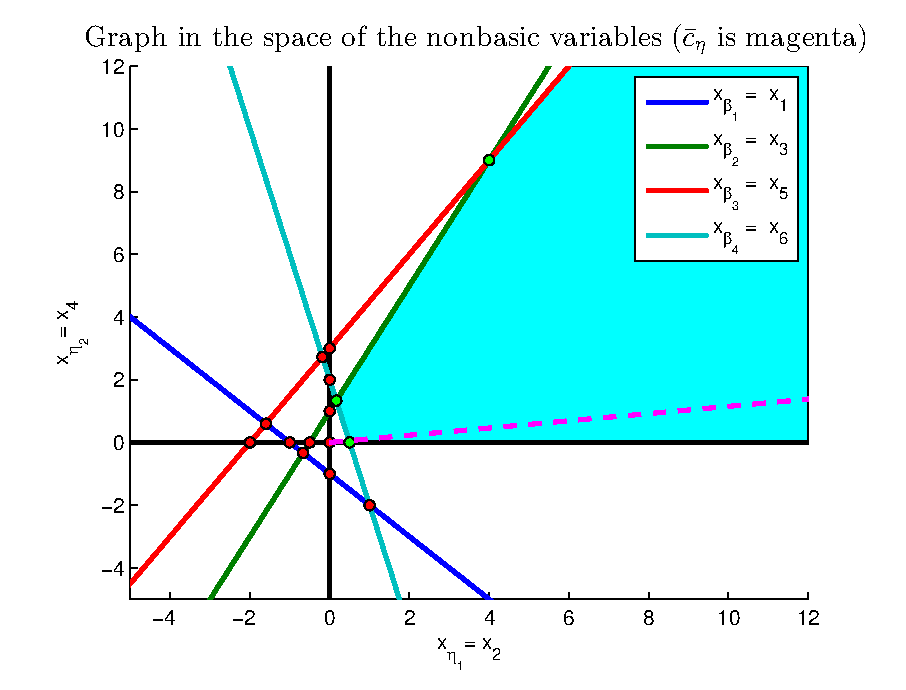
\includegraphics[width=0.5\textwidth]{p1/p1.eps}
\caption{Feasible region projected into the space of $(x_2,x_4)$}\label{fig:p1}
\end{figure}

\begin{table*}[!h]
\centering
\footnotesize
\begin{tabular}{|c|c|c|c|c|}\hline

\textbf{basic partition} & \textbf{basic feasible solution} & \textbf{basic direction} & \textbf{basic feasible direction} & $A_{\beta}^{-1}b$ \\\hline
$\beta = (1,2,4,6) $, $\eta = (3,5)$&(14,4,0,9,0,23)'&(5,2,1,3,0,11)'&(5,2,1,3,0,11)'&(14,4,9,23)'\\
&&(-3,-1,0,-2,1,-6)'&(-3,-1,0,-2,1,-6)'&\\\hline
$\beta = (1,2,4,5) $, $\eta = (3,6)$&(2.5,1/6,0,4/3,23/6,0)'&(-0.5,1/6,1,-2/3,11/6,0)'&(-0.5,1/6,1,-2/3,11/6,0)'&(2.5,1/6,4/3,23/6)'\\
&&(0.5,1/6,0,1/3,-1/6,1)'&(0.5,1/6,0,1/3,-1/6,1)'&\\\hline
$\beta = (1,2,3,5) $, $\eta = (4,6)$&(1.5,0.5,2,0,7.5,0)'&(0.75,-0.25,-1.5,1,-2.75,0)'&(0.75,-0.25,-1.5,1,-2.75,0)'&(1.5,0.5,2,7.5)'\\
&&(0.25,0.25,0.5,0,0.75,1)'&(0.25,0.25,0.5,0,0.75,1)'&\\\hline
\end{tabular}
\caption{Basic direction and basic feasible direction relative to the basic feasible solution}
\label{tab:direction}
\end{table*}

The \textbf{basic direction} and \textbf{basic feasible direction relative to the basic feasible solution} are shown in Table \ref{tab:direction}. We check whether a basic direction is a basic feasible direction by verifying  $\bar{b} = A_{\beta}^{-1}b$: $\bar{b}_i > 0$, for all $i$ such that $\bar{a}_{i,\eta_j}>0$, where $\bar{A}_{\eta_j} := A_{\beta}^{-1}A_{\eta_j}$. 

The \textbf{basic feasible rays} $\bar{z}$ are $(5,2,1,3,0,11)'$ and $(0.25,0.25,0.5,0,0.75,1)'$ as they are basic feasible directions relative to basic feasible solutions so that $A\bar{z} = \mathbf{0}$, and also $\bar{z} \geq \mathbf{0}$. Since they are basic feasible rays, they are \textbf{extreme rays} of its feasible region.